\documentclass[10pt]{article}

\usepackage[margin=0.75in]{geometry}
\usepackage{amsmath,amsthm,amssymb}
\usepackage{xcolor}
\usepackage{cancel}
\usepackage{graphicx}
\usepackage{changepage}
\usepackage{circuitikz}
\usepackage{pgfplots}
\usepackage{physics}
\usepackage{hyperref}
\usepackage{siunitx}
\usepackage{fontspec}
\usepackage{relsize}
\usepackage{subfig}
\usepackage{todonotes}
\usepackage{multicol, multirow, booktabs}
\usepackage[breakable]{tcolorbox}
\usepackage[inline]{enumitem}

\theoremstyle{definition}
\newtheorem{problem}{Problem}
\newtheorem{soln}{Solution}

\pgfplotsset{compat=newest}
\usetikzlibrary{lindenmayersystems}
\usetikzlibrary{arrows}
\usetikzlibrary{calc}
\usetikzlibrary{positioning, fit}
\usetikzlibrary{3d, perspective}

\definecolor{incolor}{HTML}{303F9F}
\definecolor{outcolor}{HTML}{D84315}
\definecolor{cellborder}{HTML}{CFCFCF}
\definecolor{cellbackground}{HTML}{F7F7F7}
\newcommand{\ui}{\hat{i}}
\newcommand{\uj}{\hat{j}}
\newcommand{\uk}{\hat{k}}
\newcommand{\ux}{\hat{x}}
\newcommand{\uy}{\hat{y}}
\newcommand{\uz}{\hat{z}}
\newcommand{\primed}[1]{#1^\prime}
\pgfdeclarelayer{background}  
\pgfsetlayers{background,main}
\AtBeginDocument{\RenewCommandCopy\qty\SI}
\newcommand{\justif}[2]{&{#1}&\text{#2}}
\DeclareMathOperator\Arg{Arg}

\makeatletter
\newcommand{\boxspacing}{\kern\kvtcb@left@rule\kern\kvtcb@boxsep}
\makeatother
\newcommand{\prompt}[4]{
    \ttfamily\llap{{\color{#2}[#3]:\hspace{3pt}#4}}\vspace{-\baselineskip}
}

\newcommand{\thevenin}[2]{
  \begin{center}
    \begin{circuitikz} \draw
      (0,0) -- (2,0) to[battery1, l_=$V_{Th}\eq#1$] (2,2) 
      to[resistor, l_=$R_{Th}\eq#2$] (0,2)
      ;
      \draw [o-] (-.07,2.079);
      \draw [o-] (-.07,0.079);
    \end{circuitikz}
  \end{center}
}

\newcommand{\norton}[2]{
  \begin{center}
    \begin{circuitikz} \draw
      (0,0) -- (3,0) to[american current source, l_=$I_{N}\eq#1$] (3,2) -- (0,2) (2,0)
      to[resistor, l=$R_{N}\eq#2$] (2,2)
      ;
      \draw [o-] (-.07,2.079);
      \draw [o-] (-.07,0.079);
    \end{circuitikz}
  \end{center}
}

\newcommand{\highlight}[1]{\colorbox{yellow}{$\displaystyle #1$}}

\newcommand{\ti}[1]{\widetilde{#1}}

\newfontface{\Kaufmann}{Kaufmann}
\DeclareTextFontCommand{\kf}{\Kaufmann}
\newcommand{\scriptr}{\fontsize{12pt}{12pt}\kf{r}}

\newfontface{\KaufmannB}{Kaufmann Bd BT}
\DeclareTextFontCommand{\kfb}{\KaufmannB}
\newcommand{\bscriptr}{\fontsize{12pt}{12pt}\kfb{r}}

\newcommand{\bv}[1]{\mathbf{#1}}

\title{Math 3770H: Assignment I}
\author{Jeremy Favro (0805980) \\ Trent University, Peterborough, ON, Canada}
\date{\today}

\begin{document}
\maketitle

% PROBLEM 1
\begin{problem}
Verify that each of the two numbers $z = 1 \pm i$ satisfies the equation $z^2 - 2z + 2 = 0$.
\end{problem}
\begin{soln}
  \begin{align*}
     & =(1 - i)^2 - 2(1 - i) + 2 \\
     & =-2i - 2 + 2i + 2         \\
     & =0
  \end{align*}
  and
  \begin{align*}
     & =(1 + i)^2 - 2(1 + i) + 2 \\
     & =2i - 2 - 2i + 2          \\
     & =0
  \end{align*}
\end{soln}

% PROBLEM 2
\begin{problem}
Prove that multiplication of complex numbers is commutative, as stated at the beginning
of Sec. 2.
\end{problem}
\begin{soln}
  \begin{proof}
    Let $a,b\in \mathbb{C}$ with $a=x_1+ iy_1$ and $b=x_2+ iy_2$ where $x_n,y_n\in \mathbb{R}$. Then,
    \begin{align*}
      a\cdot b & = (x_1+ iy_1)\cdot(x_2+ iy_2)          \\
               & = x_1x_2+ iy_1x_2 + ix_1y_2+ i^2y_1y_2 \justif{\quad}{Definition, Commutativity of addition and multiplication under $\mathbb{R}$} \\
               & = (x_1x_2-y_1y_2)+ i(x_2y_1 + x_1y_2) \justif{\quad}{Commutativity of addition and multiplication under $\mathbb{R}$}
    \end{align*}
    and
    \begin{align*}
      b\cdot a & = (x_2+ iy_2)\cdot(x_1+ iy_1)         \\
               & = x_1x_2+ix_1y_2+ix_2y_1+i^2y_1y_2 \justif{\quad}{Definition, Commutativity of addition and multiplication under $\mathbb{R}$}   \\
               & = (x_1x_2-y_1y_2)+ i(x_2y_1 + x_1y_2) \justif{\quad}{Commutativity of addition and multiplication under $\mathbb{R}$}
    \end{align*}
  \end{proof}
\end{soln}
\newpage

% PROBLEM 3
\begin{problem}
Reduce each of these quantities to a real number:\\
\begin{center}
  \begin{enumerate*}[label=(\alph*)]
    \item $\displaystyle\frac{1+2i}{3-4i}+\frac{2-i}{5i}$;\qquad~
    \item $\displaystyle\frac{5i}{(1-i)(2-i)(3-i)}$;\qquad~
    \item $\displaystyle(1-i)^4$.
  \end{enumerate*}
\end{center}
\end{problem}
\begin{soln}~
  \begin{enumerate}[label=(\alph*)]
    \item \begin{align*}
             & =\frac{1+2i}{3-4i}+\frac{2-i}{5i}                                 \\
             & =\frac{1+2i}{3-4i}\frac{3+4i}{3+4i}+\frac{2-i}{5i}\frac{-5i}{-5i} \\
             & =\frac{-5+10i}{25}+\frac{-5-10i}{25}=-2/5
          \end{align*}
    \item \begin{align*}
             & =\frac{5i}{(1-i)(2-i)(3-i)} \\
             & =\frac{5i}{-10i}=-1/2
          \end{align*}
    \item \begin{align*}
             & =(1-i)^4                 \\
             & =(\sqrt{2}e^{-i\pi/4})^4 \\
             & =(4e^{-i\pi})            \\
             & =-4
          \end{align*}
  \end{enumerate}
\end{soln}

% PROBLEM 4
\begin{problem}
Verify that $\displaystyle\sqrt{2}\abs{z}\geq \abs{\Re z} +\abs{\Im z}$
\end{problem}
\begin{soln}
  Let $z=x+iy$. Then,
  \begin{align*}
     & \sqrt{2}\abs{z}        \geq  \abs{\Re z} +\abs{\Im z}                      \\
     & \implies \sqrt{2}\sqrt{x^2+y^2}  \geq  \abs{x} +\abs{y}                    \\
     & \implies 2x^2+2y^2               \geq  \left(\abs{x} +\abs{y}\right)^2     \\
     & \implies 2x^2+2y^2 - \left(\abs{x} +\abs{y}\right)^2               \geq  0 \\
     & \implies 2x^2+2y^2 - \abs{x}^2-\abs{y}^2-2\abs{xy}               \geq  0   \\
     & \implies 2x^2+2y^2 - x^2-y^2-2\abs{xy}               \geq  0               \\
     & \implies x^2+y^2-2\abs{xy}               \geq  0                           \\
     & \implies (\abs{x}^2-\abs{y}^2)               \geq  0
  \end{align*}
\end{soln}
\newpage

% PROBLEM 5
\begin{problem}
Using the fact that $\abs{z_1-z_2}$ is the distance between two points $z_1$ and $z_2$, give a geometric
argument that $\abs{z-1}=\abs{z+i}$ represents the line through the origin whose slope is $-1$.
\end{problem}
\begin{soln}~\\
  \begin{center}
    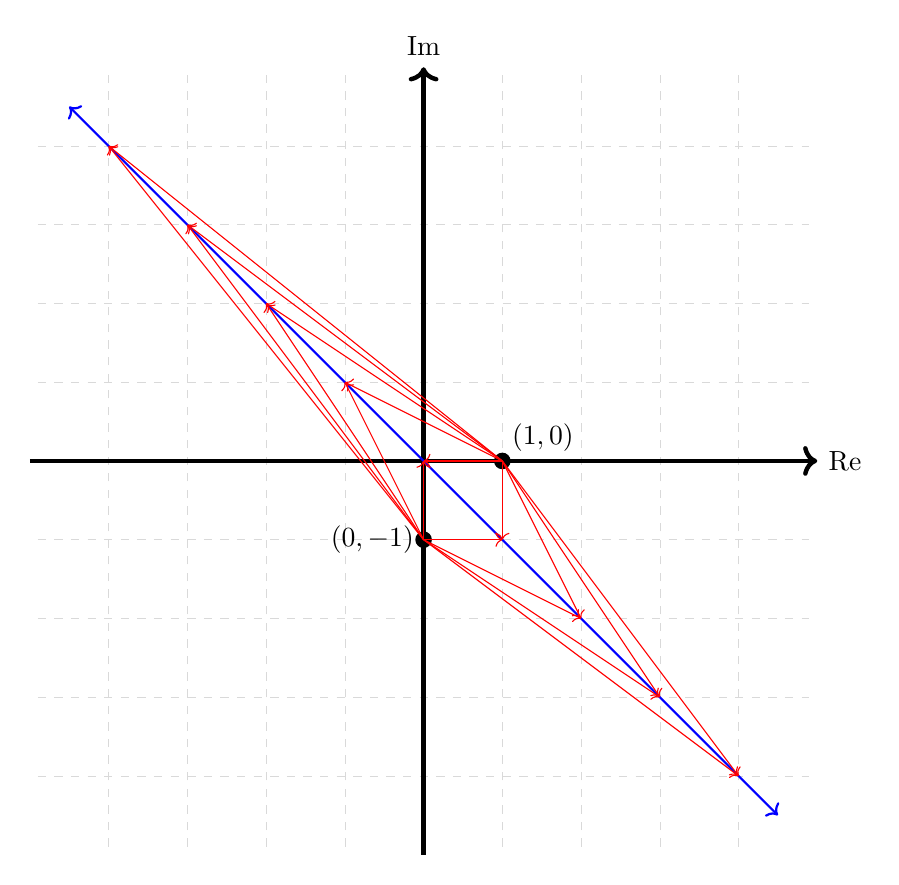
\begin{tikzpicture}
      \draw[help lines, color=gray!30, dashed] (-4.9,-4.9) grid (4.9,4.9);
      \draw[->,ultra thick] (-5,0)--(5,0) node[right]{$\Re$};
      \draw[->,ultra thick] (0,-5)--(0,5) node[above]{$\Im$};
      \draw[<->, thick, blue] (4.5,-4.5)--(-4.5,4.5);
      \fill (1,0) circle [radius=3pt] node[above right]{$(1,0)$};
      \fill (0,-1) circle [radius=3pt] node[left]{$(0,-1)$};
      \foreach \i in {-4,...,4}
        {
          \draw[->, red] (1,0) -- (\i,-\i);
          \draw[->, red] (0,-1) -- (\i,-\i);
        }
    \end{tikzpicture}
  \end{center}
  As we can see in the figure, the only points equidistant to $1$ and $-i$ are the points on the line $-x$. We can immediately recognize that the values of $z$
  will form a line when plotted as that is the only way that the distance from two fixed points can be equal.
\end{soln}

% PROBLEM 6
\begin{problem}
By factoring $z^4 - 4z^2 + 3$ into two quadratic factors and using inequality (2), Sec. 5,
show that if $z$ lies on the circle $\abs{z} = 2$, then
$$\abs{\frac{1}{z^4-4z^2+3}}\leq \frac{1}{3}$$
\end{problem}
\begin{soln}
  We begin by factoring as $z^4 - 4z^2 + 3=(z^2-1)(z^2-3)$. If we want our inequality to hold then $\abs{z^4-4z^2+3} \geq 3$
  so $\abs{(z^2-1)(z^2-3)}\geq 3$ and because $\abs{z}^2=z^2$ we can substitute in our value for $\abs{z}$ directly giving us
  \begin{align*}
     & \abs{(2^2-1)(2^2-3)}\geq 3 \\
     & \implies \abs{3}\geq 3
  \end{align*}
  and taking the reciprocal will flip the $\geq$ as we used at the beginning.
\end{soln}
\newpage

% PROBLEM 7
\begin{problem}
Find the principal argument $\Arg{z}$ when\\
\begin{center}
  \begin{enumerate*}[label=(\alph*)]
    \item $\displaystyle z=\frac{-2}{1+\sqrt{3}i}$;\qquad~
    \item $\displaystyle z=\left(\sqrt{3}-i\right)^6$.
  \end{enumerate*}
\end{center}
\end{problem}
\begin{soln}
  To do this we just need to determine the real and imaginary components and take the arctangent of $\Im/\Re$:
  \begin{enumerate}[label=(\alph*)]
    \item \begin{align*}
             & =\frac{-2}{1+\sqrt{3}i}\frac{1-\sqrt{3}i}{1-\sqrt{3}i} \\
             & =\frac{-2+2\sqrt{3}i}{4}=-1/2+\sqrt{3}i/2
          \end{align*}
          which gives $\Arg z=\arctan\left(\displaystyle\frac{\frac{\sqrt{3}}{2}}{-\frac{1}{2}}\right)=-\pi/3$ which isn't quite right when we look at the
          number on the Argand plane. This is because $\arctan$ will only give us the ``correct'' answer when our point lies in the first and fourth quadrants.
          Here this isn't the case so the actual value of $\Arg z$ is the value $\arctan$ ``would'' take on if it were defined in the quadrant we
          are currently in. This gives $\Arg z=2\pi/3$ which is the correct value.
    \item Here we can take a bit of a shortcut and notice that $\Arg z = 6 \Arg \left(\sqrt{3}-i\right)$ through properties of exponentiation when
          writing $z$ in polar form. Using this and being careful of the arctan ambiguity we get $\Arg z = \pi$
  \end{enumerate}
\end{soln}

% PROBLEM 8
\begin{problem}
Find $\left(-8-8\sqrt{3}i\right)^{1/4}$, express the roots in rectangular coordinates,
exhibit them as the vertices of a certain square, and point out which is the principal root.
\end{problem}
\begin{soln}
  \begin{align*}
     & =\left(-8-8\sqrt{3}i\right)^{1/4}                                         \\
     & =\left(16e^{i(4\pi/3+2k\pi)}\right)^{1/4}\justif{\quad}{$k\in\mathbb{Z}$} \\
     & =2e^{i(\pi/3+k\pi/2)}=1+\sqrt{3}i,-\sqrt{3}+i,-1-\sqrt{3}i,\sqrt{3}-i
  \end{align*}
  The principal root here is the case where $k=0$ which gives $1+\sqrt{3}i$.
  \begin{center}
    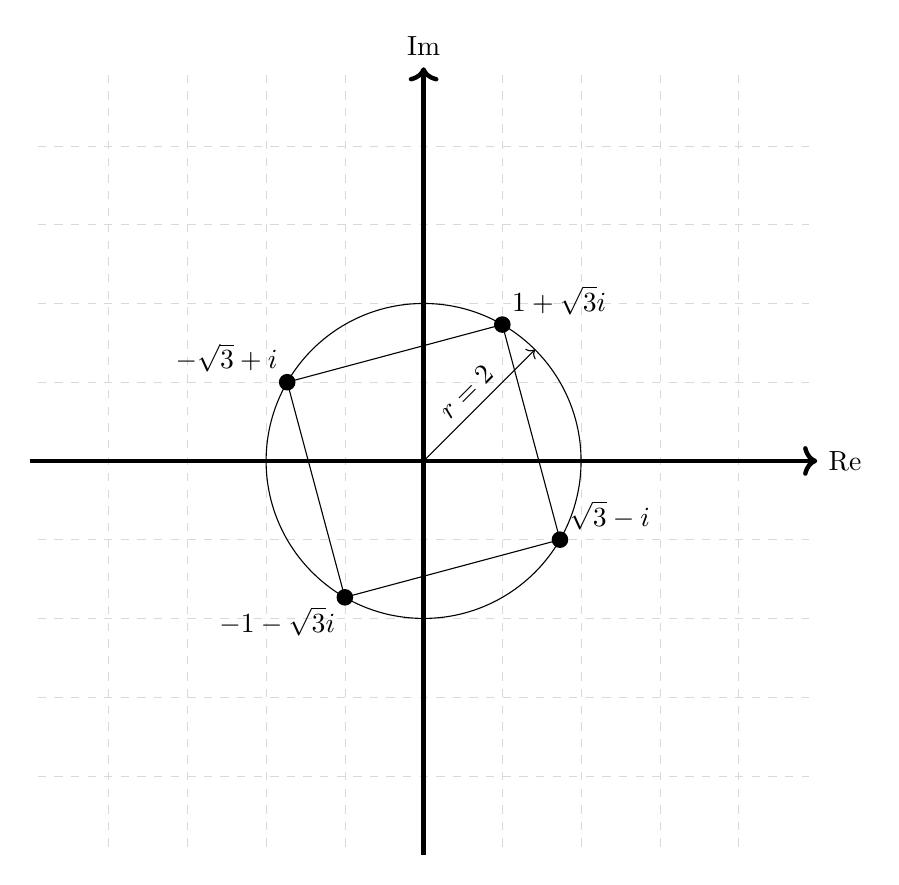
\begin{tikzpicture}
      \draw[help lines, color=gray!30, dashed] (-4.9,-4.9) grid (4.9,4.9);
      \draw[->,ultra thick] (-5,0)--(5,0) node[right]{$\Re$};
      \draw[->,ultra thick] (0,-5)--(0,5) node[above]{$\Im$};

      \coordinate(A) at (1,{sqrt(3)});
      \coordinate(B) at (-{sqrt(3)},1);
      \coordinate(C) at (-1,-{sqrt(3)});
      \coordinate(D) at ({sqrt(3)},-1);

      \fill (A) circle [radius=3pt] node[above right]{$1+\sqrt{3}i$};
      \fill (B) circle [radius=3pt] node[above left]{$-\sqrt{3}+i$};
      \fill (C) circle [radius=3pt] node[below left]{$-1-\sqrt{3}i$};
      \fill (D) circle [radius=3pt] node[above right]{$\sqrt{3}-i$};
      \draw[] (A) -- (B) -- (C) -- (D) --(A);

      \draw[] (0,0) circle[radius=2];
      \draw[->] (0,0) -- ({sqrt(2)},{sqrt(2)}) node[midway, above, rotate=45]{$r=2$};
    \end{tikzpicture}
  \end{center}
\end{soln}
\end{document}